\documentclass[
11pt, % The default document font size, options: 10pt, 11pt, 12pt
codirector, % Uncomment to add a codirector to the title page
]{charter} 




% El títulos de la memoria, se usa en la carátula y se puede usar el cualquier lugar del documento con el comando \ttitle
\titulo{Desarrollo de un dispositivo de rastreo satelital mediante GNSS (Global Navigation Satellite System)} 

% Nombre del posgrado, se usa en la carátula y se puede usar el cualquier lugar del documento con el comando \degreename
\posgrado{Carrera de Especialización en Sistemas Embebidos} 
%\posgrado{Carrera de Especialización en Internet de las Cosas} 
%\posgrado{Carrera de Especialización en Intelegencia Artificial}
%\posgrado{Maestría en Sistemas Embebidos} 
%\posgrado{Maestría en Internet de las cosas}

% Tu nombre, se puede usar el cualquier lugar del documento con el comando \authorname
\autor{Ing. Nicolás Gabriel Cettra} 

% El nombre del director y co-director, se puede usar el cualquier lugar del documento con el comando \supname y \cosupname y \pertesupname y \pertecosupname
\director{Nombre del Director}
\pertenenciaDirector{pertenencia} 
% FIXME:NO IMPLEMENTADO EL CODIRECTOR ni su pertenencia
\codirector{John Doe} % para que aparezca en la portada se debe descomentar la opción codirector en el documentclass
\pertenenciaCoDirector{FIUBA}

% Nombre del cliente, quien va a aprobar los resultados del proyecto, se puede usar con el comando \clientename y \empclientename
\cliente{Alejandro Castellano}
\empresaCliente{America GIS S.R.L.}

% Nombre y pertenencia de los jurados, se pueden usar el cualquier lugar del documento con el comando \jurunoname, \jurdosname y \jurtresname y \perteunoname, \pertedosname y \pertetresname.
\juradoUno{Nombre y Apellido (1)}
\pertenenciaJurUno{pertenencia (1)} 
\juradoDos{Nombre y Apellido (2)}
\pertenenciaJurDos{pertenencia (2)}
\juradoTres{Nombre y Apellido (3)}
\pertenenciaJurTres{pertenencia (3)}
 
\fechaINICIO{21 de junio de 2023}		%Fecha de inicio de la cursada de GdP \fechaInicioName
\fechaFINALPlan{15 de agosto de 2023} 	%Fecha de final de cursada de GdP
\fechaFINALTrabajo{15 de mayo de 2024}	%Fecha de defensa pública del trabajo final


\begin{document}

\maketitle
\thispagestyle{empty}
\pagebreak


\thispagestyle{empty}
{\setlength{\parskip}{0pt}
\tableofcontents{}
}
\pagebreak


\section*{Registros de cambios}
\label{sec:registro}


\begin{table}[ht]
\label{tab:registro}
\centering
\begin{tabularx}{\linewidth}{@{}|c|X|c|@{}}
\hline
\rowcolor[HTML]{C0C0C0} 
Revisión & \multicolumn{1}{c|}{\cellcolor[HTML]{C0C0C0}Detalles de los cambios realizados} & Fecha      \\ \hline
0      & Creación del documento                                 &\fechaInicioName \\ \hline
1      & Se completa hasta el punto 5 inclusive                 & 04 de julio de 2023 \\ \hline
2      & Se completa hasta el punto 9 inclusive                 & 10 de julio de 2023 \\ \hline
3      & Se completa hasta el punto 12 inclusive                 & 20 de julio de 2023 \\ \hline
%		  Se puede agregar algo más \newline
%		  En distintas líneas \newline
%		  Así                                                    & dd/mm/aaaa \\ \hline
%3      & Se completa hasta el punto 11 inclusive                & dd/mm/aaaa \\ \hline
%4      & Se completa el plan	                                 & dd/mm/aaaa \\ \hline
\end{tabularx}
\end{table}

\pagebreak



\section*{Acta de constitución del proyecto}
\label{sec:acta}

\begin{flushright}
Buenos Aires, \fechaInicioName
\end{flushright}

\vspace{2cm}

Por medio de la presente se acuerda con el Ing. \authorname\hspace{1px} que su Trabajo Final de la \degreename\hspace{1px} se titulará ``\ttitle'', consistirá esencialmente en la implementación de un sistema embebido que tendrá la capacidad de adquirir un posicionamiento global. Este sistema podrá comunicarse con el servidor proporcionado por la organización mediante internet. Además, contará con un acelerómetro para detectar aceleraciones repentinas en el dispositivo, un botón de propósito general y una autonomía de al menos 24 horas; y tendrá un presupuesto preliminar estimado de 612 horas de trabajo y 7065 USD, con fecha de inicio \fechaInicioName\hspace{1px} y fecha de presentación pública \fechaFinalName.

Se adjunta a esta acta la planificación inicial.

\vfill

% Esta parte se construye sola con la información que hayan cargado en el preámbulo del documento y no debe modificarla

\begin{table}[ht]
\centering
\begin{tabular}{ccc}
\begin{tabular}[c]{@{}c@{}}Dr. Ing. Ariel Lutenberg \\ Director posgrado FIUBA\end{tabular} & \hspace{2cm} & \begin{tabular}[c]{@{}c@{}}\clientename \\ \empclientename \end{tabular} \vspace{2.5cm} \\ 
\multicolumn{3}{c}{\begin{tabular}[c]{@{}c@{}} \supname \\ Director del Trabajo Final\end{tabular}} \vspace{2.5cm} \\
%\begin{tabular}[c]{@{}c@{}}\jurunoname \\ Jurado del Trabajo Final\end{tabular}     &  & \begin{tabular}[c]{@{}c@{}}\jurdosname\\ Jurado del Trabajo Final\end{tabular}  \vspace{2.5cm}  \\
%\multicolumn{3}{c}{\begin{tabular}[c]{@{}c@{}} \jurtresname\\ Jurado del Trabajo Final\end{tabular}} \vspace{.5cm}                                                                     
\end{tabular}
\end{table}


\section{1. Descripción técnica-conceptual del proyecto a realizar}
\label{sec:descripcion}


Con el objetivo de ofrecer soluciones más específicas de manera flexible y económica, se desarrollará un sistema embebido que permitirá adquirir un posicionamiento global a través de un módulo GNSS. Este sistema se comunicará con el servidor proporcionado por la organización mediante GPRS. Además, contará con un acelerómetro para detectar aceleraciones bruscas en el dispositivo. También se incluirá un botón con funciones programables de propósito múltiple y una autonomía de al menos 24 horas.

Una de las características clave que se debe tener en cuenta es la capacidad de adaptar el hardware a diferentes sectores. Para el desarrollo de este dispositivo, se utilizará el módulo GNSS/GPRS A9G de la empresa Ai Thinker, al que se le acoplará el hardware necesario para cumplir con los objetivos planteados. Es importante mencionar que se cuenta con el SDK del módulo, lo que permitirá programarlo según las necesidades.

El dispositivo debe ser capaz de enviar información a través de GPRS utilizando los protocolos de comunicación UDP o TCP, y se requerirá la capacidad de utilizar MQTT dentro del protocolo TCP. Dicha comunicación se puede apreciar en la figura 1. Además, se utilizará el acelerómetro MPU6050 mediante la interfaz I2C para la adquisición de aceleraciones.

En cuanto a la alimentación del dispositivo, se utilizará una batería de 3,7 V. Esto hace que la eficiencia energética sea indispensable para maximizar la duración de la batería.

En cuanto al botón, este debe ser multiproposito. El dispositivo generará un evento al pulsarlo y el significado será asignado del lado del servidor.

El software embebido debe ser diseñado teniendo en cuenta la posibilidad de agregar módulos adicionales en el futuro, y se implementará un sistema operativo en tiempo real (RTOS). Además, se utilizará como base para futuros proyectos.

En la figura 1 se puede apreciar el diagrama en bloque de la comunicacion entre el dispositivo y el servidor.


\begin{figure}[htpb]
\centering 
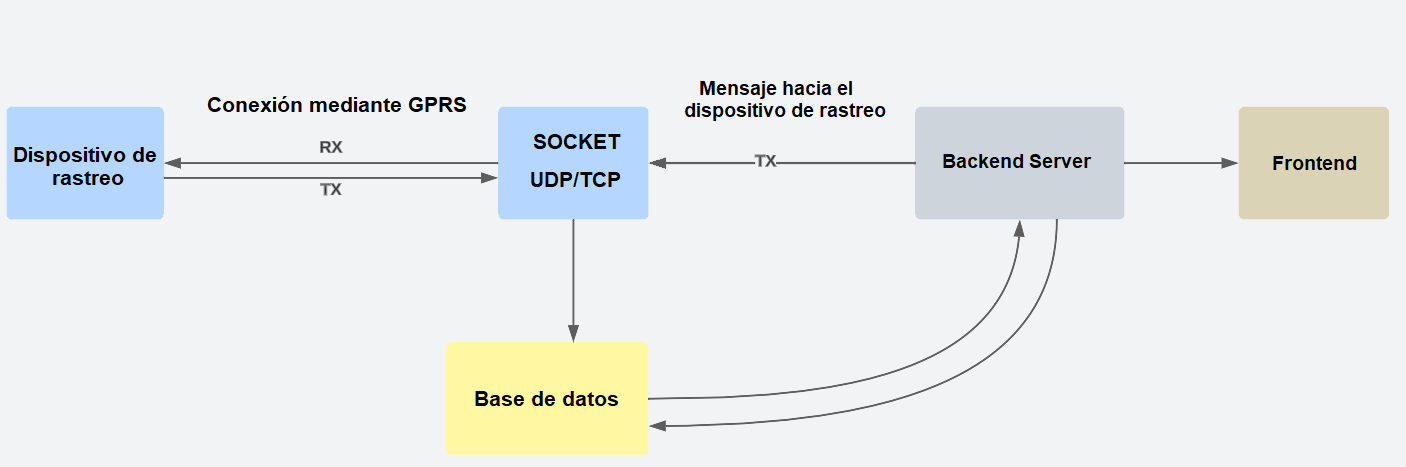
\includegraphics[width=1\textwidth]{./Figuras/diagBloque.png}
\caption{Diagrama en bloques del sistema.}
\label{fig:diagBloques}
\end{figure}

\vspace{30px}
\pagebreak
\section{2. Identificación y análisis de los interesados}
\label{sec:interesados}


\begin{table}[ht]
%\caption{Identificación de los interesados}
%\label{tab:interesados}
\begin{tabularx}{\linewidth}{@{}|l|X|X|l|@{}}
\hline
\rowcolor[HTML]{C0C0C0} 
Rol           & Nombre y Apellido & Organización 	& Puesto 	\\ \hline
Cliente       & \clientename      &\empclientename	&    Gerente    	\\ \hline
Responsable   & \authorname       & FIUBA        	& Alumno 	\\ \hline
Orientador    & \supname	      & \pertesupname 	& Director Trabajo final \\ \hline
\end{tabularx}
\end{table}

\section{3. Propósito del proyecto}
\label{sec:proposito}


El propósito de este proyecto es desarrollar un sistema embebido que permita controlar un hardware de adquisición de datos, en particular enfocado en el posicionamiento global. Se busca que este sistema tenga la capacidad de adaptarse a diferentes sectores, brindando flexibilidad y versatilidad en su aplicación. Además, se busca lograr una solución más económica en comparación con otras alternativas disponibles en el mercado. El enfoque central es garantizar la adaptabilidad del hardware y reducir los costos asociados al desarrollo y despliegue del sistema.


\section{4. Alcance del proyecto}
\label{sec:alcance}

El sistema embebido a desarrollar tendrá los siguientes alcances: \\

El proyecto incluye:
\begin{itemize}

    \item Implementación en RTOS de bibliotecas para la interpretación de tramas GPS y el protocolo de comunicación con control CRC (verificación por redundancia cíclica).
    \item Desarrollo de protocolo para el envio de reportes gatillados por eventos.
    \item Kit de comandos para configurar el dispositivo mediante USB, GPRS o SMS.
    \item El software sea capaz de establecer una conexión a Internet mediante GPRS para el intercambio de información via UDP/TCP.
    \item El software sea capaz de gestionar reportes en memoria en caso de interrupciones en la conexión a Internet.
    \item Elaboración de manuales de usuario, guías rápidas de uso y otros materiales de documentación.

\end{itemize}
El proyecto no incluye:
\begin{itemize}
    \item Desarrollo del hardware.
    \item Calibraciones y certificaciones.
    \item Despliegue de la red de cobertura de la señal.
\end{itemize}
\pagebreak

\section{5. Supuestos del proyecto}
\label{sec:supuestos}
Para el desarrollo del presente proyecto se supone que:
\begin{itemize}
\item Se supone que la empresa proporcionará el hardware necesario, incluyendo la tarjeta SIM para la conexión GPRS y la interfaz de programación del dispositivo.
\item Se asume que el módulo GNSS en condiciones óptimas, tiene una tolerancia de error de 10 metros en la precisión de la posición.
\item Se supone que el dispositivo solo funcionará si hay una antena compatible con 2G dentro de su rango de alcance.
\end{itemize}

\section{6. Requerimientos}
\label{sec:requerimientos}

\begin{enumerate}
\item Requerimientos funcionales
    \begin{enumerate}
    \item El sistema debe ser capaz de adquirir el posicionamiento global mediante un módulo GNSS.
    \item El sistema debe comunicarse con el servidor proporcionado por la empresa America GIS a través de GPRS.
    \item El dispositivo debe contar con un acelerómetro para detectar aceleraciones abruptas.
    \item El sistema debe tener un botón de propósito general con funcionalidad programable.
    \item El sistema debe tener una autonomía mínima de 24 horas.
    \item El sistema debe generar reportes temporizados.
    \item El sistema debe generar reportes en función de eventos particulares, como presionar el botón multipropósito, una aceleración abrupta o un cambio de dirección.
    \item El sistema debe ser configurable mediante USB, GPRS o SMS.
    \item El dispositivo debe conectarse a Internet mediante GPRS para el intercambio de información.
    \item El sistema debe ser capaz de comunicarse utilizando los protocolos UDP o TCP.
    \item El sistema debe ser capaz de almacenar reportes en memoria en caso de intermitencia en la conexión a Internet.
    \end{enumerate}

\item Requerimientos de documentación
    \begin{enumerate}
    \item Se debe proporcionar documentación detallada del proceso de configuración del sistema.
    \item Se debe incluir documentación del hardware utilizado, incluyendo el módulo GNSS, el acelerómetro y el botón multipropósito.
    \item Se debe proporcionar documentación del SDK del módulo GNSS/GPRS A9G de Ai Thinker.
    \item Se debe incluir una guía de usuario que explique el funcionamiento y las características del sistema.
    \item Se debe documentar el protocolo de comunicación utilizado para la interacción con el servidor de America GIS.
    \item Se debe proporcionar una documentación clara sobre las especificaciones y limitaciones del sistema, incluyendo la tolerancia de error del módulo GNSS y la dependencia de una antena compatible con 2G.
    \item Se debe proporcionar una memoria del trabajo.
    \item Se debe proporcionar un registro de avances.
    \end{enumerate}
\end{enumerate}

\section{7. Historias de usuarios (\textit{Product backlog})}
\label{sec:backlog}

En esta sección se presentarán las historias de usuario, y cada una de ellas recibirá una puntuación basada en tres aspectos:
\begin{itemize}
 \item Dificultad: Representa la cantidad de trabajo necesario para completar la historia de usuario.
 \item Complejidad: Indica la complejidad del trabajo requerido para cumplir con la historia de usuario.
 \item Riesgo: Refleja el nivel de incertidumbre asociado con el trabajo necesario para la historia de usuario.
\end{itemize}
Se utilizará una escala basada en la serie de Fibonacci, donde los números mayores implicarán un mayor costo en términos de tiempo y recursos. Si la suma de los tres componentes no corresponde a un número de la serie de Fibonacci, se elegirá el número más cercano en la serie como puntuación asignada.

\begin{itemize}
    \item Como usuario, quiero poder configurar la frecuencia de generación de reportes temporizados para adaptarla a mis necesidades. (Ponderación: 5 story points)
    \begin{itemize}
        \item Dificultad: 2 (Moderada)
        \item Complejidad: 2 (Moderada)
        \item Riesgo: 1 (Bajo)
    \end{itemize}    
    
    \item Como usuario, quiero recibir notificaciones inmediatas en caso de detectar una aceleración abrupta en el dispositivo para poder tomar medidas rápidamente. (Ponderación: 10 story points)
    \begin{itemize}
        \item Dificultad: 3 (Compleja)
        \item Complejidad: 3 (Compleja)
        \item Riesgo: 4 (Alto)
    \end{itemize}    

    
    \item Como usuario, quiero poder personalizar la funcionalidad del botón multipropósito para adaptarlo a mis necesidades específicas. (Ponderación: 3 story points)
    \begin{itemize}
        \item Dificultad: 1 (Baja)
        \item Complejidad: 1 (Baja)
        \item Riesgo: 1 (Baja)
    \end{itemize}    

    
    \item Como usuario, quiero tener la opción de enviar los reportes de manera automática al servidor de America GIS a través del protocolo UDP para una comunicación más eficiente. (Ponderación: 8 story points)
    \begin{itemize}
        \item Dificultad: 2 (Moderada)
        \item Complejidad: 3 (Compleja)
        \item Riesgo: 3 (Moderado)
    \end{itemize}  
    
    \item Como usuario, quiero poder almacenar los reportes en memoria en caso de pérdida temporal de conexión a Internet para asegurar que no se pierda información importante. (Ponderación: 6 story points)
    \begin{itemize}
        \item Dificultad: 2 (Moderada)
        \item Complejidad: 2 (Moderada)
        \item Riesgo: 2 (Moderado)
    \end{itemize}  

    
    \item Como usuario, quiero recibir una notificación en tiempo real cuando se produzca un cambio de dirección brusco en el dispositivo para estar al tanto de cualquier evento inesperado. (Ponderación: 8 story points)
    \begin{itemize}
        \item Dificultad: 2 (Moderada)
        \item Complejidad: 3 (Compleja)
        \item Riesgo: 3 (Moderado)
    \end{itemize}  
    
    \item Como usuario, quiero tener la posibilidad de configurar el sistema mediante una interfaz sencilla y amigable a través de USB para facilitar la configuración y personalización. (Ponderación: 5 story points)
    \begin{itemize}
        \item Dificultad: 2 (Moderada)
        \item Complejidad: 2 (Moderada)
        \item Riesgo: 1 (Bajo)
    \end{itemize}  
    
    \item Como usuario, quiero poder consultar la documentación detallada del sistema para comprender mejor su funcionamiento y aprovechar al máximo sus características. (Ponderación: 3 story points)
    \begin{itemize}
        \item Dificultad: 1 (Baja)
        \item Complejidad: 1 (Baja)
        \item Riesgo: 1 (Bajo)
    \end{itemize}  
\end{itemize}


\section{8. Entregables principales del proyecto}
\label{sec:entregables}

Los entregables del proyecto son:
\begin{itemize}
    \item Manual de uso.
    \item Código fuente del firmware.
    \item Archivo binario para actualizar el dispositivo.
    \item Informe final.
\end{itemize}


\section{9. Desglose del trabajo en tareas}
\label{sec:wbs}


\begin{enumerate}
    \item Configuración inicial del entorno de desarrollo.
    \begin{enumerate}
        \item Instalación y configuración del software de desarrollo. (12 h)
        \item Configuración del entorno de programación y depuración. (12 h)
        \item Configuración del entorno de pruebas y simulación. (12 h)
    \end{enumerate}
    
    \item Desarrollo del módulo de adquisición de posicionamiento.
    \begin{enumerate}
        \item Investigación del módulo GNSS. (30 h)
        \item Implementación de la comunicación con el módulo GNSS. (30 h)
        \item Integración de la funcionalidad de posicionamiento en el sistema embebido. (36 h)
    \end{enumerate}
    
    \item Desarrollo del módulo de detección de aceleraciones abruptas.
    \begin{enumerate}
        \item Investigación del modulo acelerómetro. (24 h)
        \item Implementación de la lectura y procesamiento de datos del acelerómetro. (24 h)
        \item Integración de la detección de aceleraciones en el sistema embebido. (30 h)
    \end{enumerate}
    
    \item Desarrollo del módulo de configuración y personalización.
    \begin{enumerate}
        \item Diseño de la interfaz de configuración mediante USB. (24 h)
        \item Implementación de la comunicación y la lógica de configuración. (30 h)
        \item Pruebas y depuración de la funcionalidad de configuración. (24 h)
    \end{enumerate}
    
    \item Desarrollo del módulo de generación y envío de reportes.
    \begin{enumerate}
        \item Diseño e implementación de la generación de reportes temporizados. (36 h)
        \item Implementación de GPIO y la lógica de configuración (18h)
        \item Desarrollo de la lógica para generar reportes en función de eventos. (30 h)
        \item Implementación de la comunicación con el servidor de America GIS. (36 h)
    \end{enumerate}
    
    \item Pruebas y validación del sistema completo.
    \begin{enumerate}
        \item Realización de pruebas de integración y validación del sistema embebido. (54 h)
        \item Pruebas de conectividad y comunicación con el servidor. (24 h)
        \item Pruebas de rendimiento y estabilidad del sistema. (24 h)
    \end{enumerate}
    
    \item Documentación del manual.
    \begin{enumerate}
        \item Elaboración del manual de usuario. (24 h)
        \item Revisión y edición del manual de usuario. (12 h)
    \end{enumerate}
    
    \item Elaboración del informe.
    \begin{enumerate}
        \item Recopilación y análisis de los resultados del proyecto. (24 h)
        \item Redacción del informe final. (30 h)
        \item Revisión y edición del informe final. (12 h)
    \end{enumerate}
\end{enumerate}

Cantidad total de horas estimadas: 612 h

\pagebreak
\section{10. Diagrama de Activity On Node}
\label{sec:AoN}

\begin{figure}[htpb]
\centering 
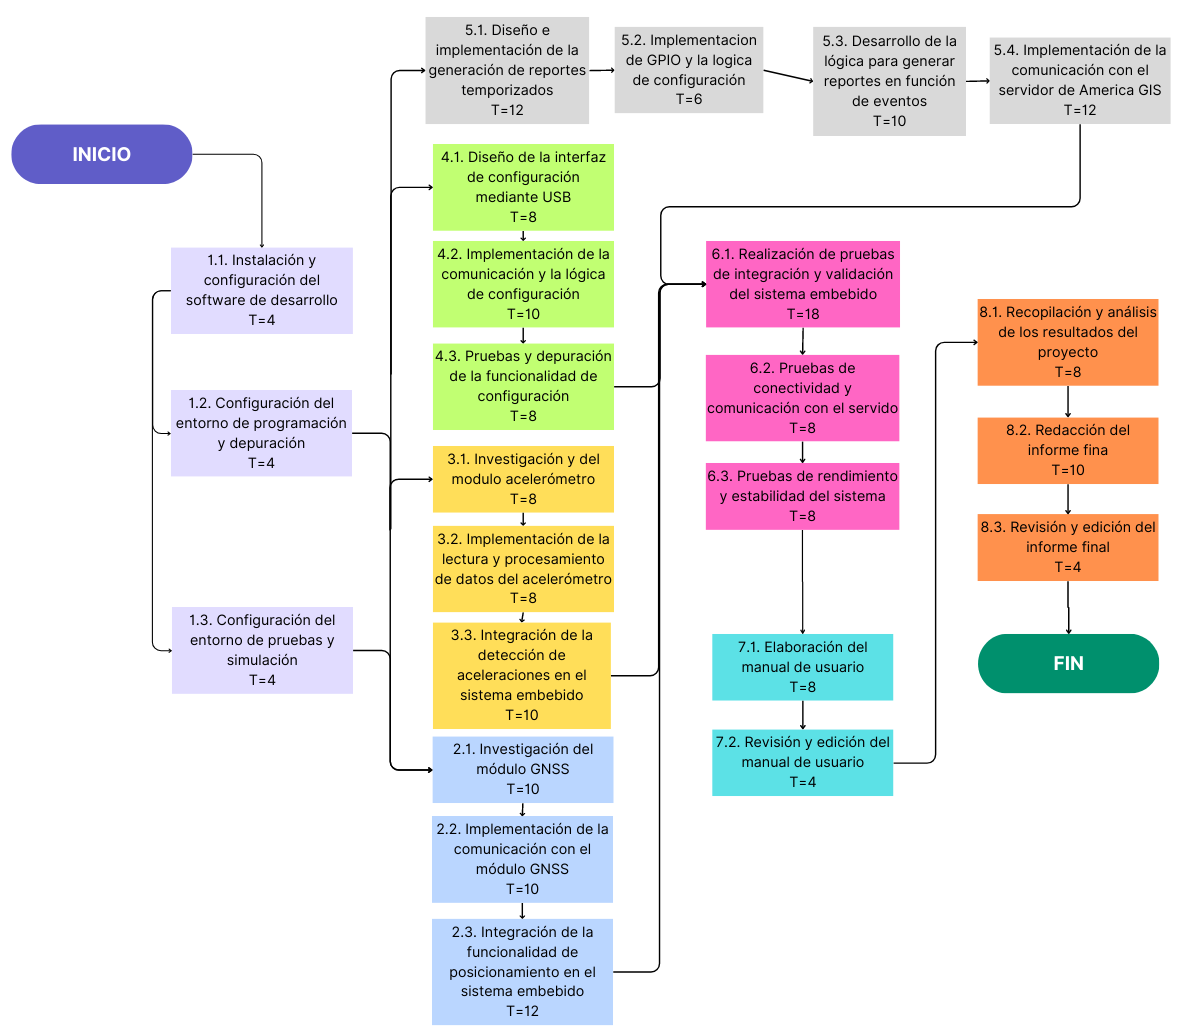
\includegraphics[width=.88\textwidth]{./Figuras/diagrama1.png}
\caption{Diagrama de \textit{Activity on Node}.}
\label{fig:AoN}
\end{figure}

\begin{figure}[htpb]
\centering 
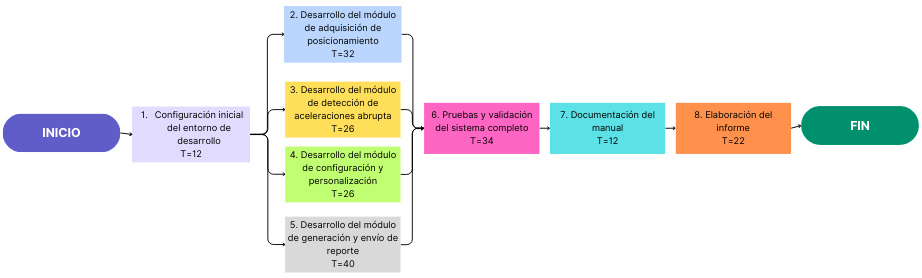
\includegraphics[width=.94\textwidth]{./Figuras/diagrama2.png}
\caption{Diagrama de \textit{Activity on Node agrupado}.}
\label{fig:AoN}
\end{figure}
\pagebreak

\section{11. Diagrama de Gantt}
\label{sec:gantt}
\begin{figure}[htpb]
\centering 
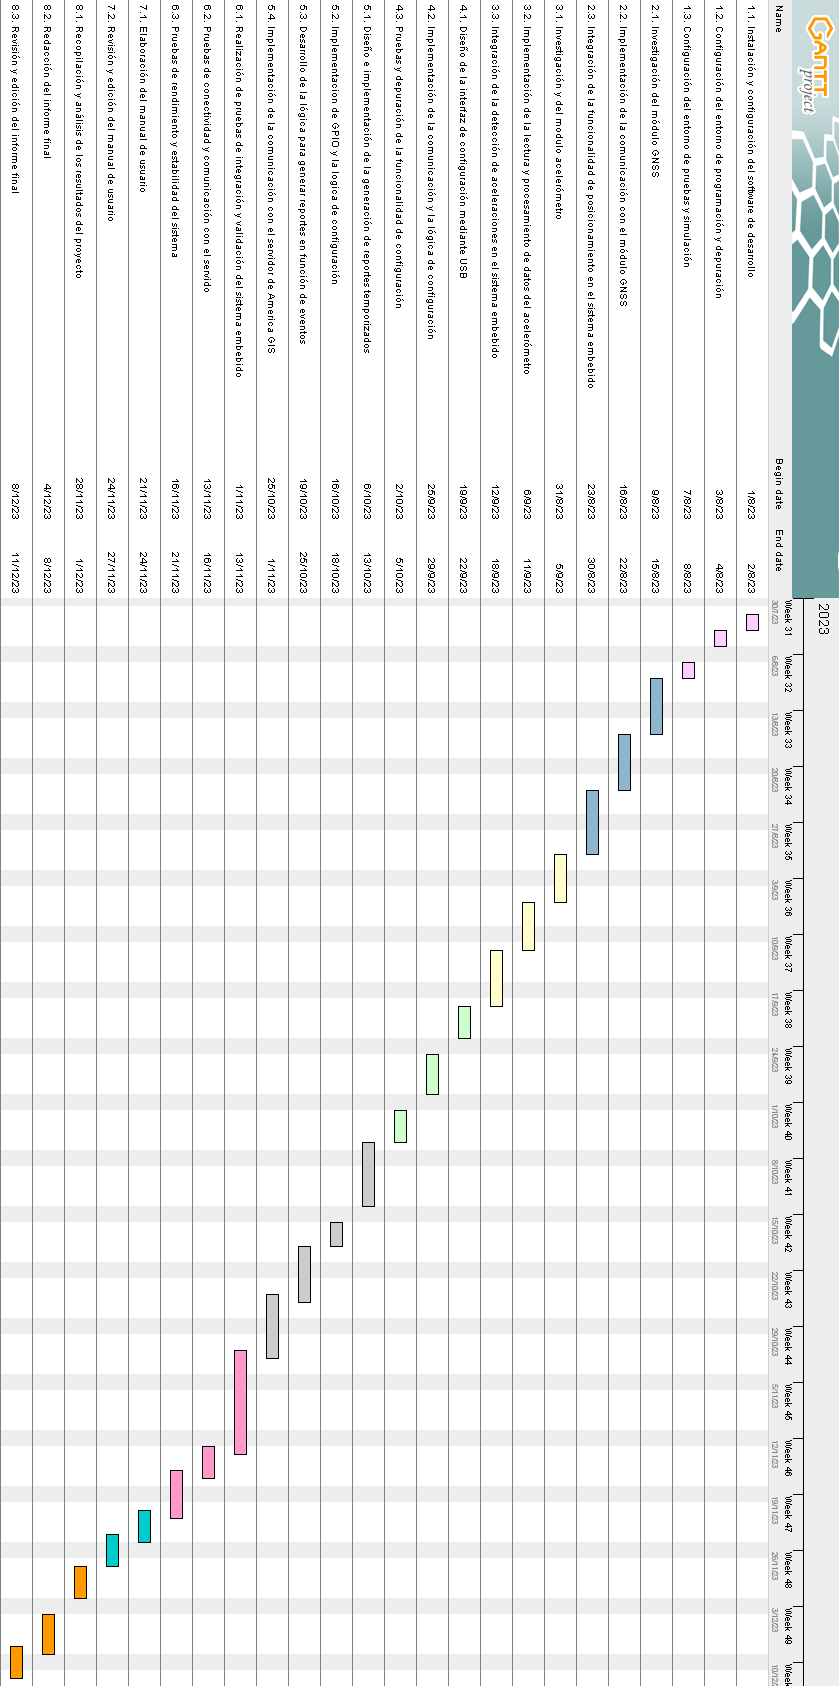
\includegraphics[height=0.78\textheight]{./Figuras/gantt_rotado.png}

\label{fig:diagGantt}
\end{figure}



\begin{landscape}

\end{landscape}


\section{12. Presupuesto detallado del proyecto}
\label{sec:presupuesto}

Los costos se encuentran expresados en USD.
\begin{table}[htpb]
\centering
\begin{tabularx}{\linewidth}{@{}|X|c|r|r|@{}}
\hline
\rowcolor[HTML]{C0C0C0} 
\multicolumn{4}{|c|}{\cellcolor[HTML]{C0C0C0}COSTOS DIRECTOS} \\ \hline
\rowcolor[HTML]{C0C0C0} 
Descripción &
  \multicolumn{1}{c|}{\cellcolor[HTML]{C0C0C0}Cantidad} &
  \multicolumn{1}{c|}{\cellcolor[HTML]{C0C0C0}Valor unitario} &
  \multicolumn{1}{c|}{\cellcolor[HTML]{C0C0C0}Valor total} \\ \hline
  \multicolumn{1}{|l|}{Dispositivo de rastreo}
 &
  \multicolumn{1}{c|}{ 1 } &
  \multicolumn{1}{c|}{ 30 } &
  \multicolumn{1}{c|}{ 30 } \\ \hline
  \multicolumn{1}{|l|}{Kit de desarrollo}
 &
  \multicolumn{1}{c|}{1} &
  \multicolumn{1}{c|}{20} &
  \multicolumn{1}{c|}{20} \\ \hline
  \multicolumn{1}{|l|}{Horas de ingenieria}
 &
  \multicolumn{1}{c|}{612} &
  \multicolumn{1}{c|}{8} &
  \multicolumn{1}{c|}{4896} \\ \hline
  \multicolumn{1}{|l|}{Componentes electrónicos varios}
 &
  \multicolumn{1}{c|}{-} &
  \multicolumn{1}{c|}{-} &
  \multicolumn{1}{c|}{100} \\ \hline
\multicolumn{3}{|c|}{SUBTOTAL} &
  \multicolumn{1}{c|}{5046} \\ \hline
\rowcolor[HTML]{C0C0C0} 
\multicolumn{4}{|c|}{\cellcolor[HTML]{C0C0C0}COSTOS INDIRECTOS} \\ \hline
\rowcolor[HTML]{C0C0C0} 
Descripción &
  \multicolumn{1}{c|}{\cellcolor[HTML]{C0C0C0}Cantidad} &
  \multicolumn{1}{c|}{\cellcolor[HTML]{C0C0C0}Valor unitario} &
  \multicolumn{1}{c|}{\cellcolor[HTML]{C0C0C0}Valor total} \\ \hline
\multicolumn{1}{|l|}{Estimado global (40\% de costos directos)} 
   &
   \multicolumn{1}{c|}{-} & 
   \multicolumn{1}{c|}{-} &
   \multicolumn{1}{c|}{2019} &\hline

\multicolumn{3}{|c|}{SUBTOTAL} &
  \multicolumn{1}{c|}{2019} \\ \hline
\rowcolor[HTML]{C0C0C0}
\multicolumn{3}{|c|}{TOTAL} &
   \multicolumn{1}{c|}{7065} \\ \hline
\end{tabularx}%
\end{table}


\section{13. Gestión de riesgos}
\label{sec:riesgos}

\begin{consigna}{red}
a) Identificación de los riesgos (al menos cinco) y estimación de sus consecuencias:
 
Riesgo 1: detallar el riesgo (riesgo es algo que si ocurre altera los planes previstos de forma negativa)
\begin{itemize}
	\item Severidad (S): mientras más severo, más alto es el número (usar números del 1 al 10).\\
	Justificar el motivo por el cual se asigna determinado número de severidad (S).
	\item Probabilidad de ocurrencia (O): mientras más probable, más alto es el número (usar del 1 al 10).\\
	Justificar el motivo por el cual se asigna determinado número de (O). 
\end{itemize}   

Riesgo 2:
\begin{itemize}
	\item Severidad (S): 
	\item Ocurrencia (O):
\end{itemize}

Riesgo 3:
\begin{itemize}
	\item Severidad (S): 
	\item Ocurrencia (O):
\end{itemize}


b) Tabla de gestión de riesgos:      (El RPN se calcula como RPN=SxO)

\begin{table}[htpb]
\centering
\begin{tabularx}{\linewidth}{@{}|X|c|c|c|c|c|c|@{}}
\hline
\rowcolor[HTML]{C0C0C0} 
Riesgo & S & O & RPN & S* & O* & RPN* \\ \hline
       &   &   &     &    &    &      \\ \hline
       &   &   &     &    &    &      \\ \hline
       &   &   &     &    &    &      \\ \hline
       &   &   &     &    &    &      \\ \hline
       &   &   &     &    &    &      \\ \hline
\end{tabularx}%
\end{table}

Criterio adoptado: 
Se tomarán medidas de mitigación en los riesgos cuyos números de RPN sean mayores a...

Nota: los valores marcados con (*) en la tabla corresponden luego de haber aplicado la mitigación.

c) Plan de mitigación de los riesgos que originalmente excedían el RPN máximo establecido:
 
Riesgo 1: plan de mitigación (si por el RPN fuera necesario elaborar un plan de mitigación).
  Nueva asignación de S y O, con su respectiva justificación:
  - Severidad (S): mientras más severo, más alto es el número (usar números del 1 al 10).
          Justificar el motivo por el cual se asigna determinado número de severidad (S).
  - Probabilidad de ocurrencia (O): mientras más probable, más alto es el número (usar del 1 al 10).
          Justificar el motivo por el cual se asigna determinado número de (O).

Riesgo 2: plan de mitigación (si por el RPN fuera necesario elaborar un plan de mitigación).
 
Riesgo 3: plan de mitigación (si por el RPN fuera necesario elaborar un plan de mitigación).

\end{consigna}


\section{14. Gestión de la calidad}
\label{sec:calidad}

\begin{consigna}{red}
Elija al menos diez requerientos que a su criterio sean los más importantes/críticos/que aportan más valor y para cada uno de ellos indique las acciones de verificación y validación que permitan asegurar su cumplimiento.

\begin{itemize} 
\item Req \#1: copiar acá el requerimiento.

\begin{itemize}
	\item Verificación para confirmar si se cumplió con lo requerido antes de mostrar el sistema al cliente. Detallar 
	\item Validación con el cliente para confirmar que está de acuerdo en que se cumplió con lo requerido. Detallar  
\end{itemize}

\end{itemize}

Tener en cuenta que en este contexto se pueden mencionar simulaciones, cálculos, revisión de hojas de datos, consulta con expertos, mediciones, etc.  Las acciones de verificación suelen considerar al entregable como ``caja blanca'', es decir se conoce en profundidad su funcionamiento interno.  En cambio, las acciones de validación suelen considerar al entregable como ``caja negra'', es decir, que no se conocen los detalles de su funcionamiento interno.

\end{consigna}

\section{15. Procesos de cierre}    
\label{sec:cierre}

\begin{consigna}{red}
Establecer las pautas de trabajo para realizar una reunión final de evaluación del proyecto, tal que contemple las siguientes actividades:

\begin{itemize}
	\item Pautas de trabajo que se seguirán para analizar si se respetó el Plan de Proyecto original:
	 - Indicar quién se ocupará de hacer esto y cuál será el procedimiento a aplicar. 
	\item Identificación de las técnicas y procedimientos útiles e inútiles que se emplearon, y los problemas que surgieron y cómo se solucionaron:
	 - Indicar quién se ocupará de hacer esto y cuál será el procedimiento para dejar registro.
	\item Indicar quién organizará el acto de agradecimiento a todos los interesados, y en especial al equipo de trabajo y colaboradores:
	  - Indicar esto y quién financiará los gastos correspondientes.
\end{itemize}

\end{consigna}


\end{document}
